\documentclass[border=0.5cm]{standalone}
\usepackage{tikz}
\usepackage{amsmath}
\usetikzlibrary{calc, angles, quotes}

\begin{document}
\begin{minipage}{.6\textwidth}
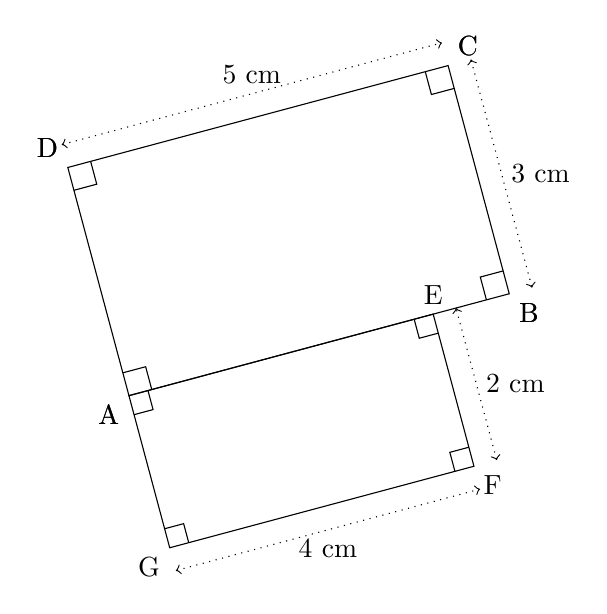
\begin{tikzpicture}
    \begin{scope}[rotate=15]
    \draw (0,0) coordinate (A) -- 
          ++(5,0) coordinate (B) -- 
          ++(0,3) coordinate (C) -- 
          ++(-5,0) coordinate (D) -- cycle;
    \foreach \p/\q/\r in {B/A/D,A/D/C,D/C/B,C/B/A} {
        \pic [draw, -, angle radius=0.3cm, angle eccentricity=1.6] {right angle=\p--\q--\r};
    }
    \foreach \p/\l in {A/below left,B/below right,C/above right,D/above left} {
        \node[\l] at (\p) {\p};
    }
    
    % Add the second rectangle
    \draw (A) -- ++(4,0) coordinate (E) --
            ++(0,-2) coordinate (F) -- 
            ++(-4,0) coordinate (G) -- cycle;
    \foreach \p/\q/\r in {G/A/E,A/E/F,E/F/G,F/G/A} {
        \pic [draw, -, angle radius=0.25cm, angle eccentricity=1.6] {right angle=\p--\q--\r};
    }
    \foreach \point/\position in {A/below left, B/below right, C/above right, D/above left, E/above, F/below right, G/below left} {
        \node[\position] at (\point) {\point};
    }
    
    % Add arrows to indicate lengths
    \draw[<->, dotted] ($(D)!0.0!(C)$) ++(-0.0cm,+0.3cm) -- ++(5cm,0) node[midway,above] {5 cm};
    \draw[<->, dotted] ($(C)!0.0!(E)$) ++(0.3cm,-0.0cm) -- ++(0,-3cm) node[midway,right] {3 cm};
    \draw[<->, dotted] ($(G)!0.0!(F)$) ++(-0.0cm,-0.3cm) -- ++(4cm,0) node[midway,below] {4 cm};
    \draw[<->, dotted] ($(F)!0.0!(G)$) ++(0.3cm,0.0cm) -- ++(0,2cm) node[midway,right] {2 cm};
    
    \end{scope}
\end{tikzpicture}
\end{minipage}%
\begin{minipage}{.4\textwidth}
\begin{align*}
\text{Perimeter of rectangle ABCD} &= 2*(\text{l} + \text{w}) \\
\text{} &= 2*(5 \text{cm} + 3 \text{cm})  \\
\text{} &= 16 \text{cm}
\end{align*}
\begin{align*}
\text{Perimeter of rectangle GFEA} &= 2*(\text{l} + \text{w}) \\
\text{} &= 2*(4 \text{cm} + 2 \text{cm})  \\
\text{} &= 12 \text{cm}
\end{align*}
\begin{align*}
\text{Total Perimeter} &= \overline{AD} + \overline{DC} + \overline{CB} + \overline{BE} + \overline{EF} + \overline{FG} + \overline{GA}\\
\text{} &= 3 \text{cm} + 5 \text{cm}  + 3 \text{cm}  + 1 \text{cm}  + 2 \text{cm}  + 4 \text{cm}  + 2 \text{cm}  \\
\text{} &= 20 \text{cm}
\end{align*}
\end{minipage}

\end{document}
